\documentclass[article.tex]{subfiles}
\begin{document}

\begin{figure}[p]
  \centering
  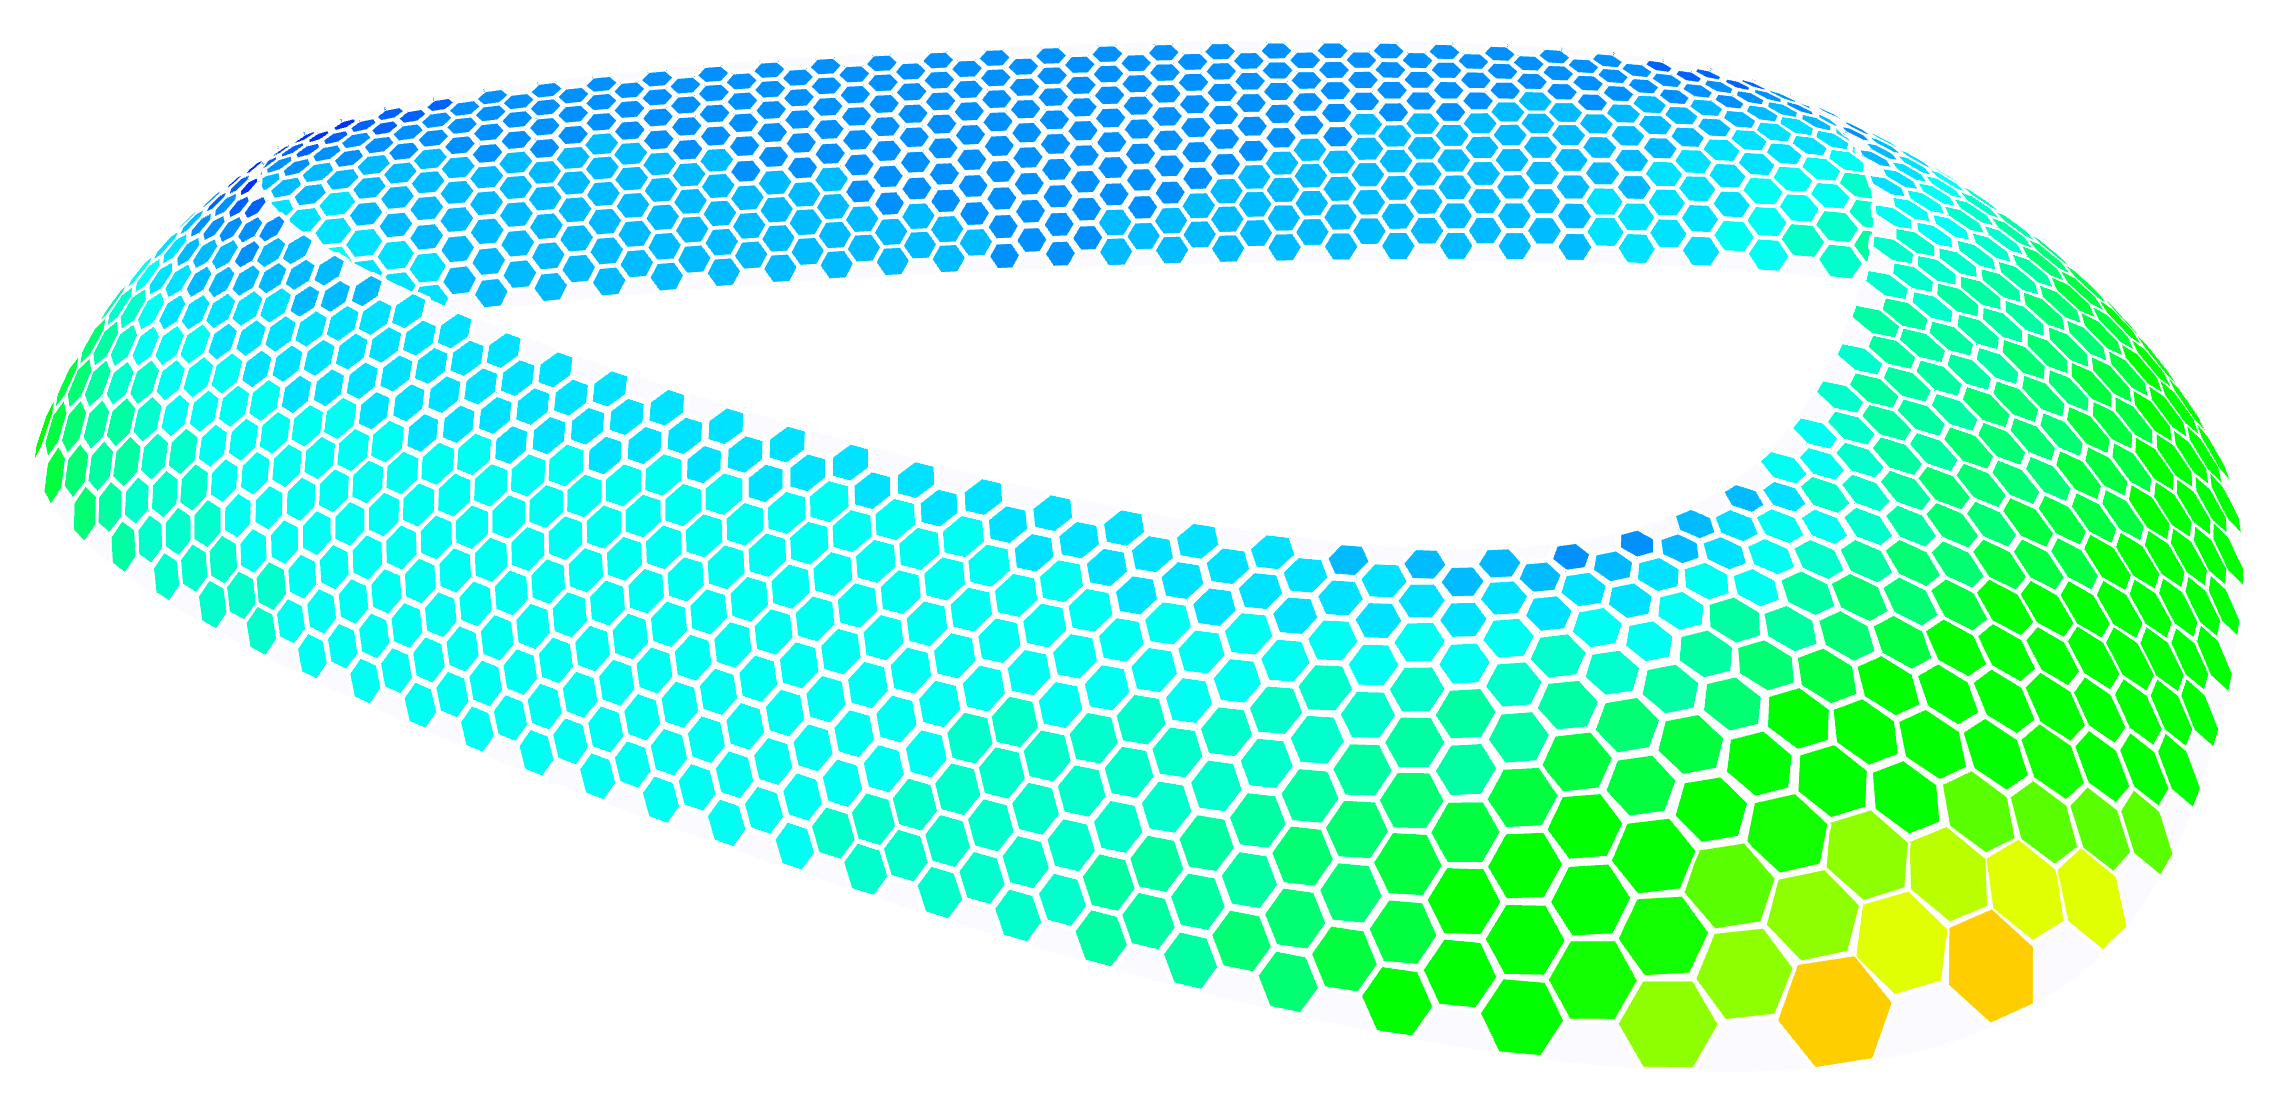
\includegraphics[width=.89\textwidth]{images/quantized_aligned5.png}
  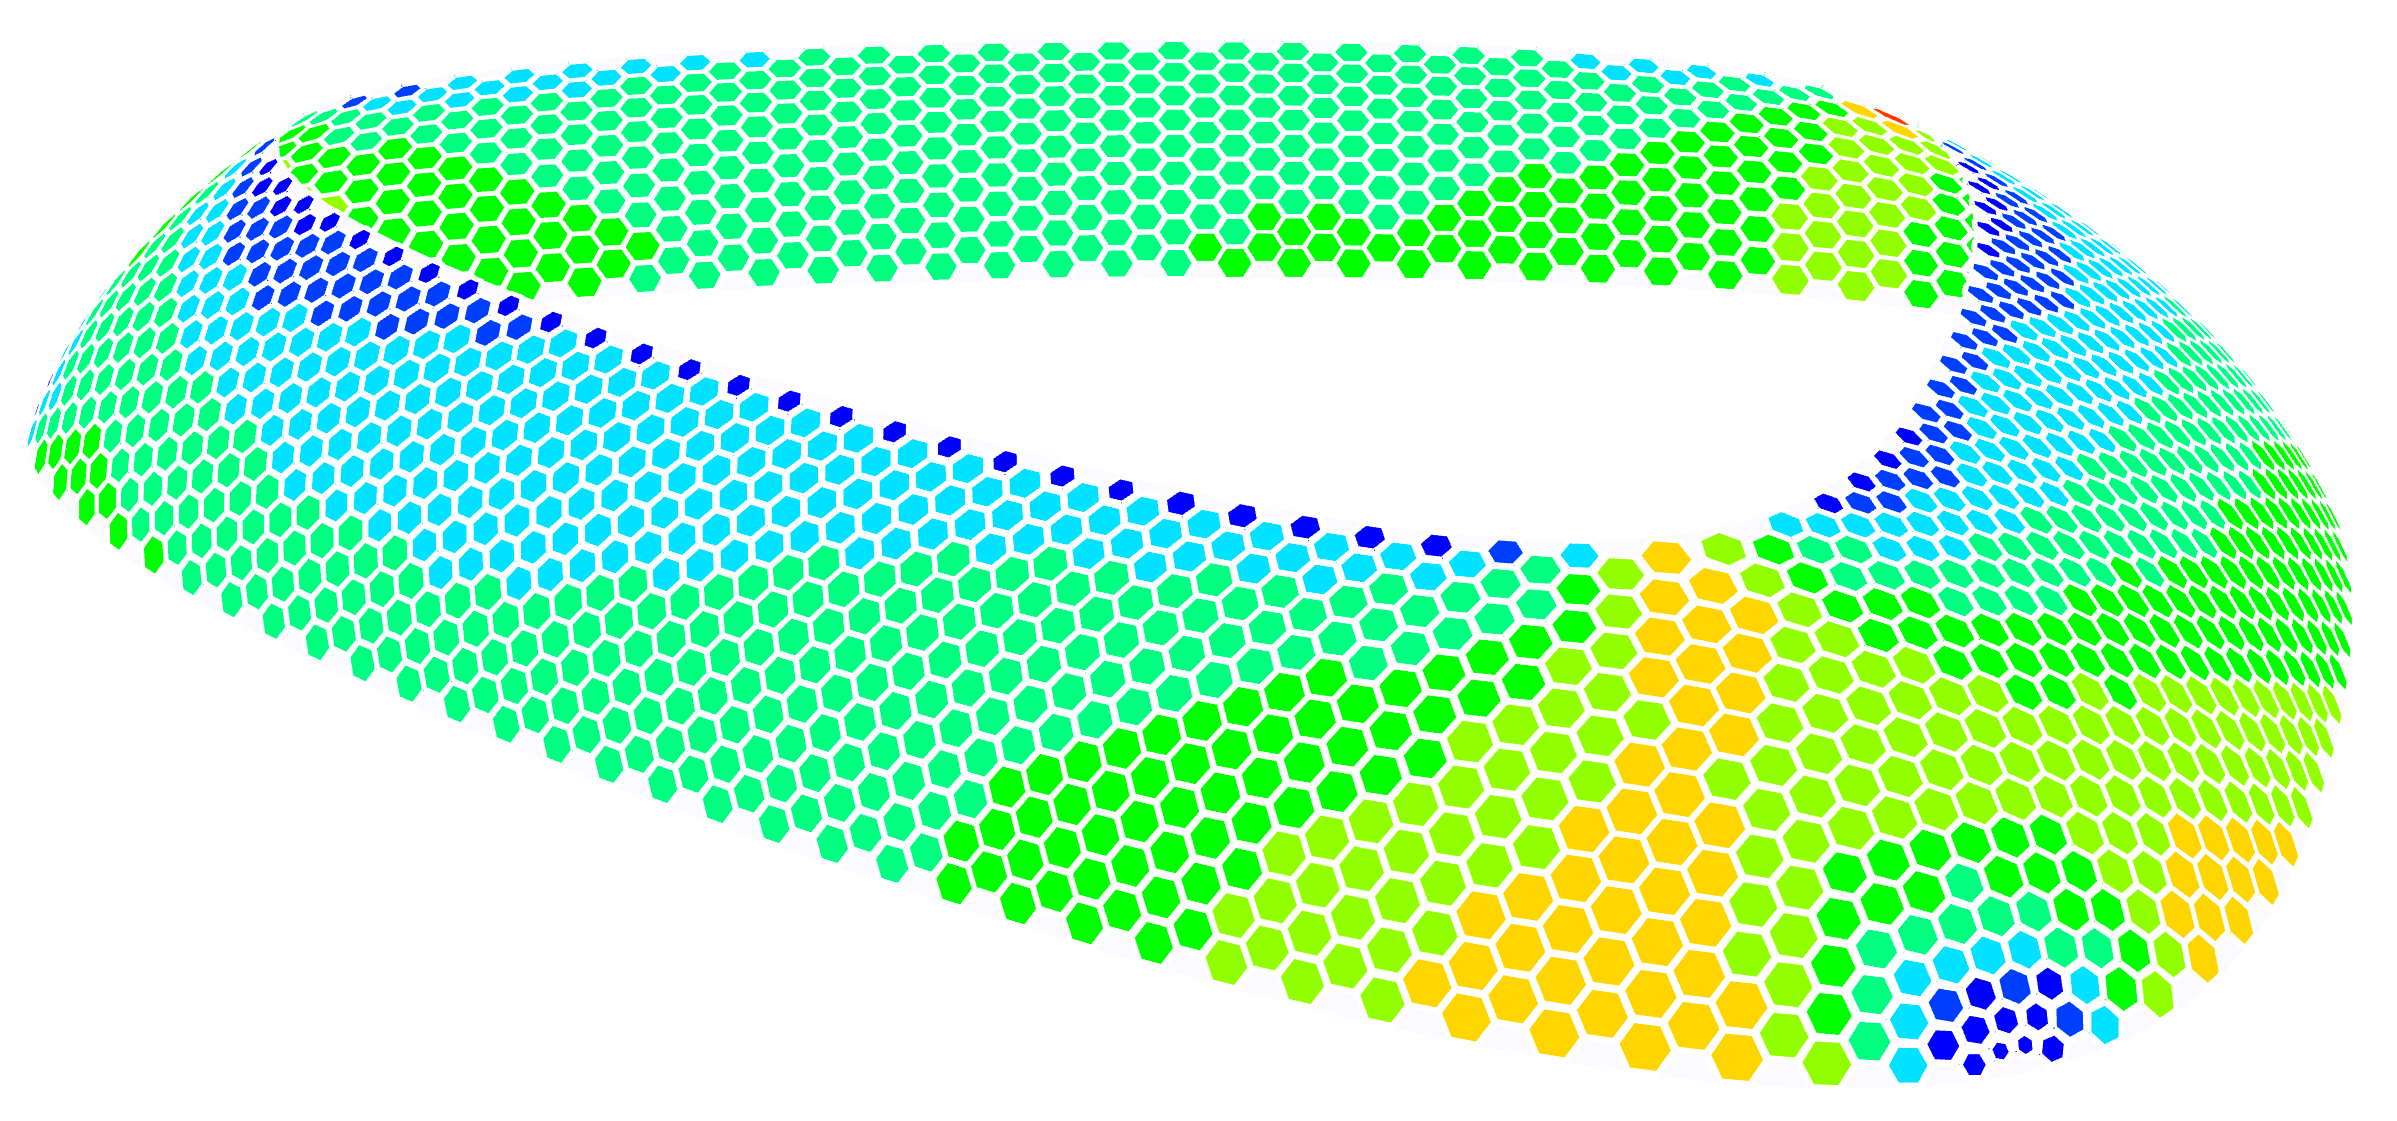
\includegraphics[width=.89\textwidth]{images/quantized_singularities5.png}
  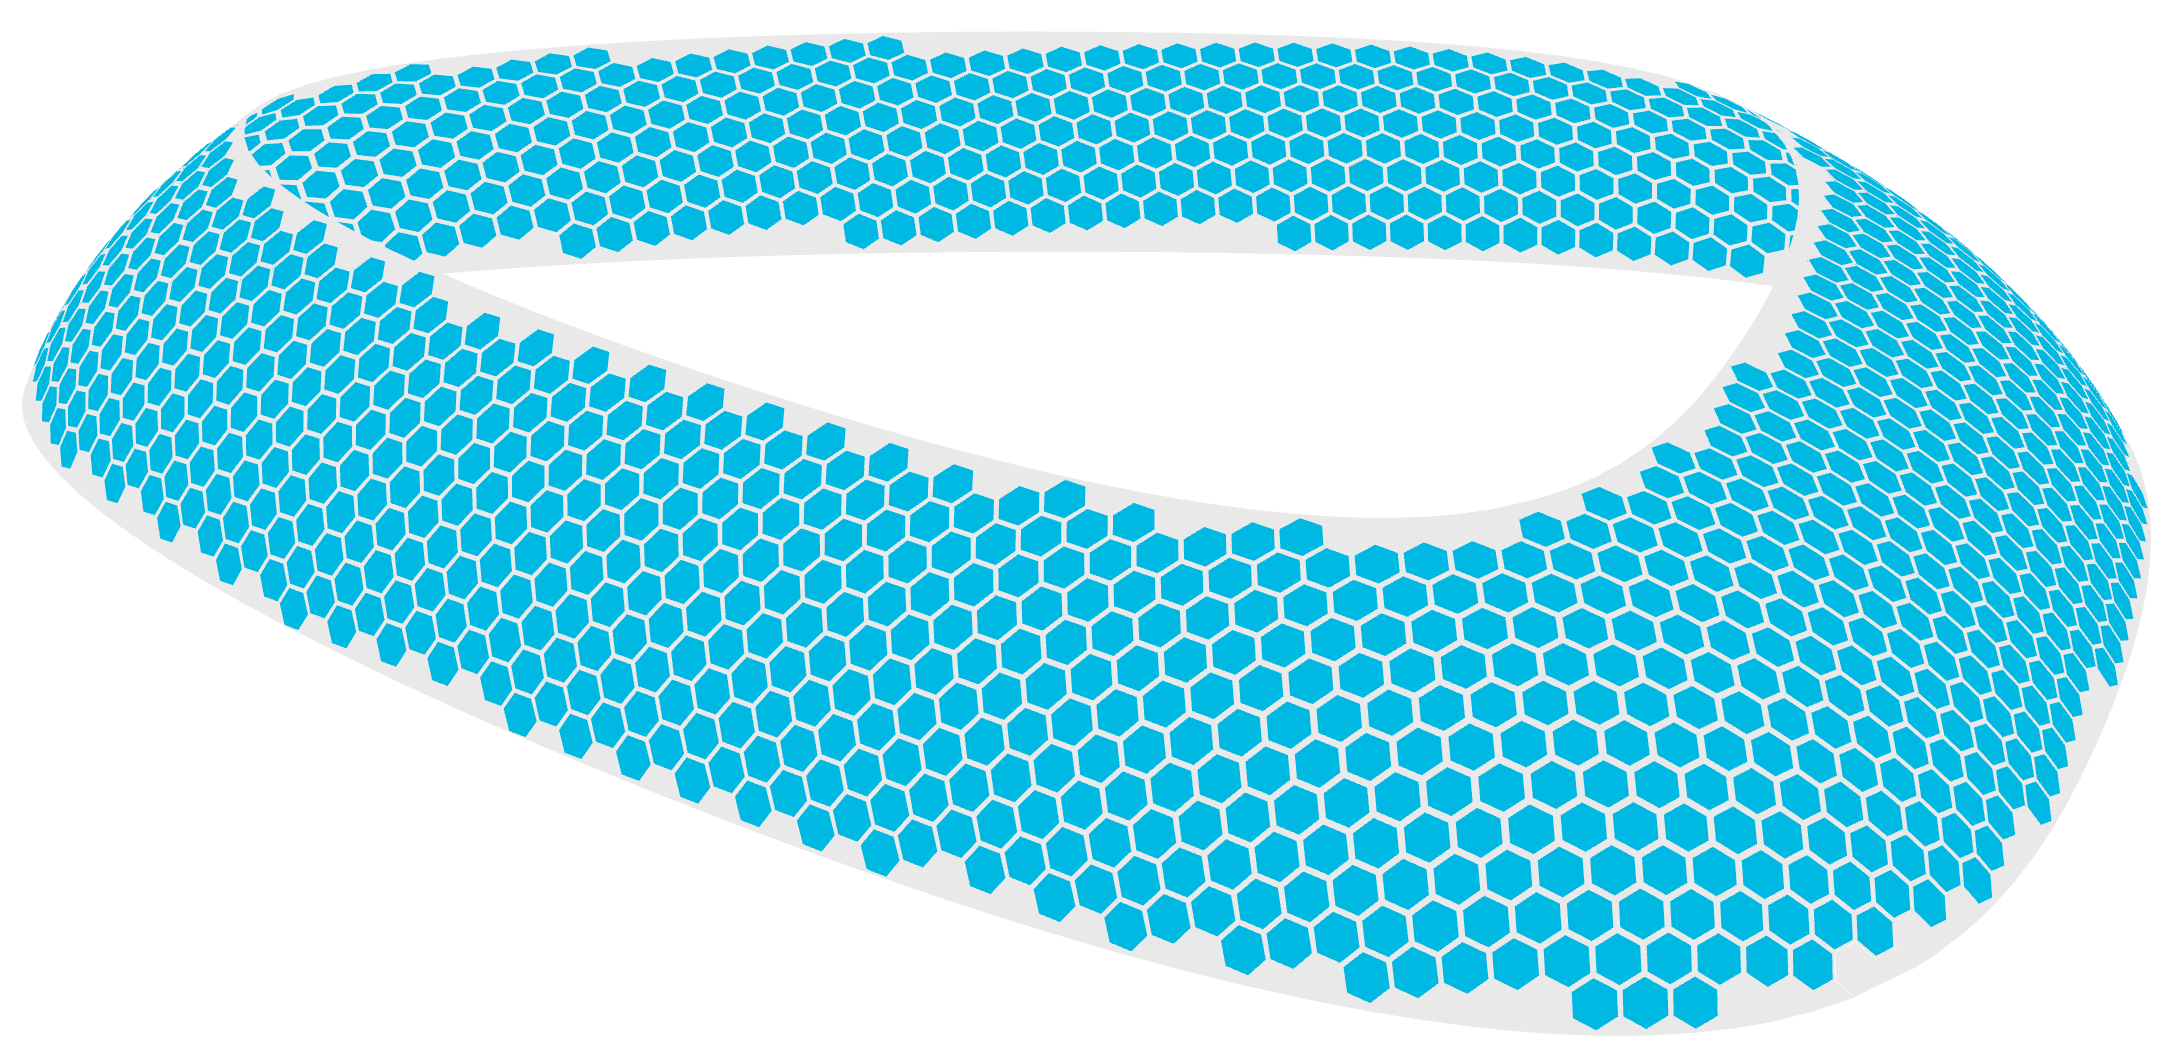
\includegraphics[width=.89\textwidth]{images/quantized_isometric2.png}
  \caption{Quantized periodic hexagonal panelizations. Boundary
    conditions affect the amount of stretch in the interior of the
    surface. Top: Hexagonal pattern aligns with the boundary, a strong
    condition that produces large deviation of panel sizes. Middle:
    Map to a pattern-adapted polygon on a cone of revolution. The
    pattern contains exceptional points at the boundary. The stretch
    is minimized while at the same time the pattern alignes with the
    boundary.  Bottom: Conformal map with the least stretch in the
    interior, pattern can be optimized to consist of congruent
    hexagons alone. In each image, panels with the same colors are
    congruent. The corresponding domains of parameterization are shown
    in Figure~\ref{fig:cone_maps_teaser}.}
  \label{fig:hex_example}
\end{figure}

\subsection{Periodic boundary conditions}
\label{sec:boundary}

If we want to construct periodic conformal maps we are allowed
to specify angle sums~$\theta_v$ at boundary vertices. The condition
for the sums of boundary angles differs from the simply-connected case in the
following way: The curvature at a boundary vertex~$v$ is given by
$\kappa_v = \pi -\theta_v$, where $\theta_v$ is the angle sum of the
adjacent triangles in the target mesh. For the two boundary loops
$(v_1, \ldots, v_n)$ and $(w_1, \ldots, w_m)$ we have:
\begin{equation}
\sum_{i=1}^n \kappa_{v_i} + \sum_{j=1}^m \kappa_{w_j} = 0. \label{eq:theta}
\end{equation}
This condition makes sure that the two boundary curves ``bend'' the
same amount and can hence be wrapped around a cone. 
We will now show how boundary conditions can be
used to construct periodic patterns on the studied models. We start
with a discrete conformal map of the doubly-curved model from Figure~\ref{fig:teaser} 
to a standard cylinder. 

\subsubsection{Straight cylinder.}
The simplest way to generate a map to the cylinder is to set the
target angles for all boundary vertices to~$\pi$. Hence the curvatures
at the boundary vertices are zero and the two boundary loops are
mapped to ``straight'' curves. 
In this case both angle sums of Equation~\eqref{eq:theta}
vanish and the target mesh can be wrapped around a cylinder, see 
Figure~\ref{fig:cone_maps_teaser}, left. The new edge lengths
computed with the variational principle correspond to the lengths on a
cylinder. This cylinder can be unrolled into the plane preserving angles
and lengths. Therefore the two boundary polygons are mapped to straight lines
in the plane. These two straight lines have to be parallel and of
equal lengths.
%
If the lengths of the boundary curves in the original model differ a
lot, then a map to a cylinder induces a lot of conformal stretch. This stretch
can be reduced by specifying special boundary conditions for a
parameterization on a cone of revolution.

\subsubsection{Cone of revolution.}
As long as Equation~\eqref{eq:theta} is satisfied we obtain a map to a
general cone of revolution. In our case, we require that the
periodic parameterization is adapted to the target pattern. 
This means that the two sums of Equation~\eqref{eq:theta} need to 
be (the same) multiples of
$\tfrac{\pi}{3}$ (triangle or hex) or multiples of $\tfrac{\pi}{2}$
(quad). We present two methods to achieve this requirement: a uniform
distribution and a concentration of curvature.

If the boundary of the mesh should align with the pattern,
then boundary angles need to be quantized, i.e., multiples of
$\tfrac{\pi}{3}$ or~$\tfrac{\pi}{2}$ need to be chosen as target
angles. In Figure~\ref{fig:cone_maps_teaser}, middle, three vertices
of the top and bottom boundary curve were manually assigned to
$\tfrac{4}{3}\pi$ and~$\tfrac{2}{3}\pi$, respectively. All other
boundary angles are set to~$\pi$, i.e., straight.  Such a map can
be used as a starting point to obtain a tesselation with quantized
hexagons as described in Section~\ref{sec:regular_hexagons}.

It is known that a discrete confomal map that does not change the lengths of the 
boundary edges exhibits the least stretch in the interior of the surface.
To obtain such a parameterization we first construct a periodic conformal 
mapping onto an
arbitrary cone such that the lengths of the boundary edges are equal. The resulting angle sums at boundary vertices of the
target mesh determine the cone angle~$\varphi$ of the map. The cone angle of
a pattern adapted periodic parameterization is the closest multiple of the 
desired quantization. We distribute the difference to the closest
quantized angle uniformly to the individual boundary vertices and
recompute the map with these angle conditions. The obtained map is 
periodic and exhibits the lowest stretch of all periodic conformal maps (see
Figure~\ref{fig:cone_maps_teaser}, right).  

\begin{figure}[bt]
  \centering
  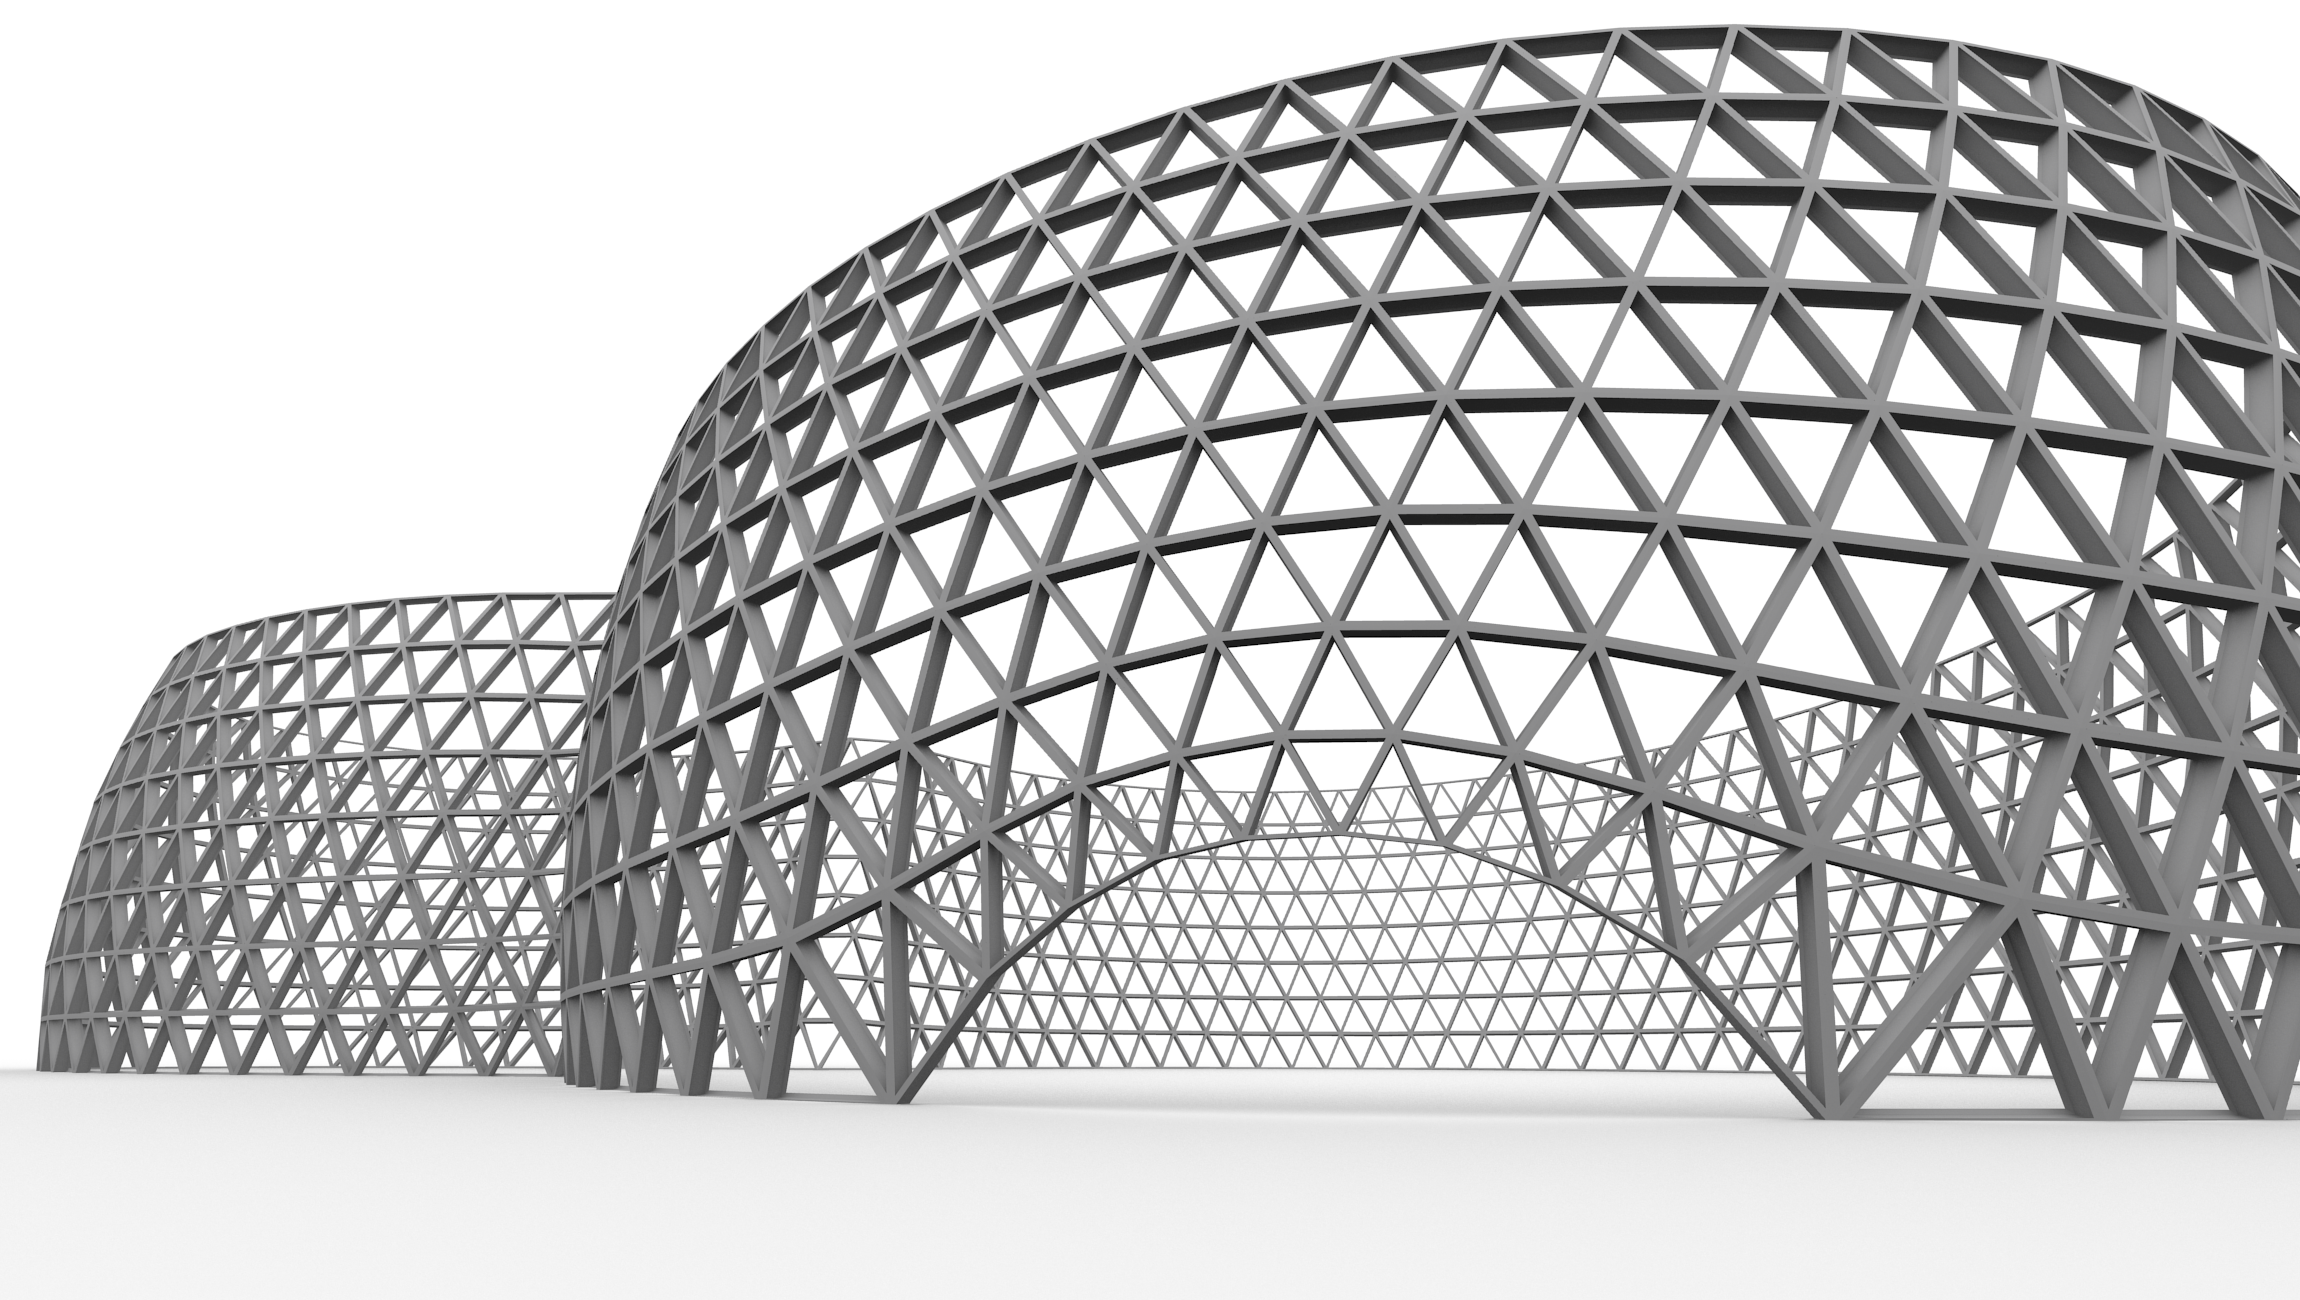
\includegraphics[width=.52\linewidth]{images/wanda_entrances2.png}
  \hspace{.5cm}
  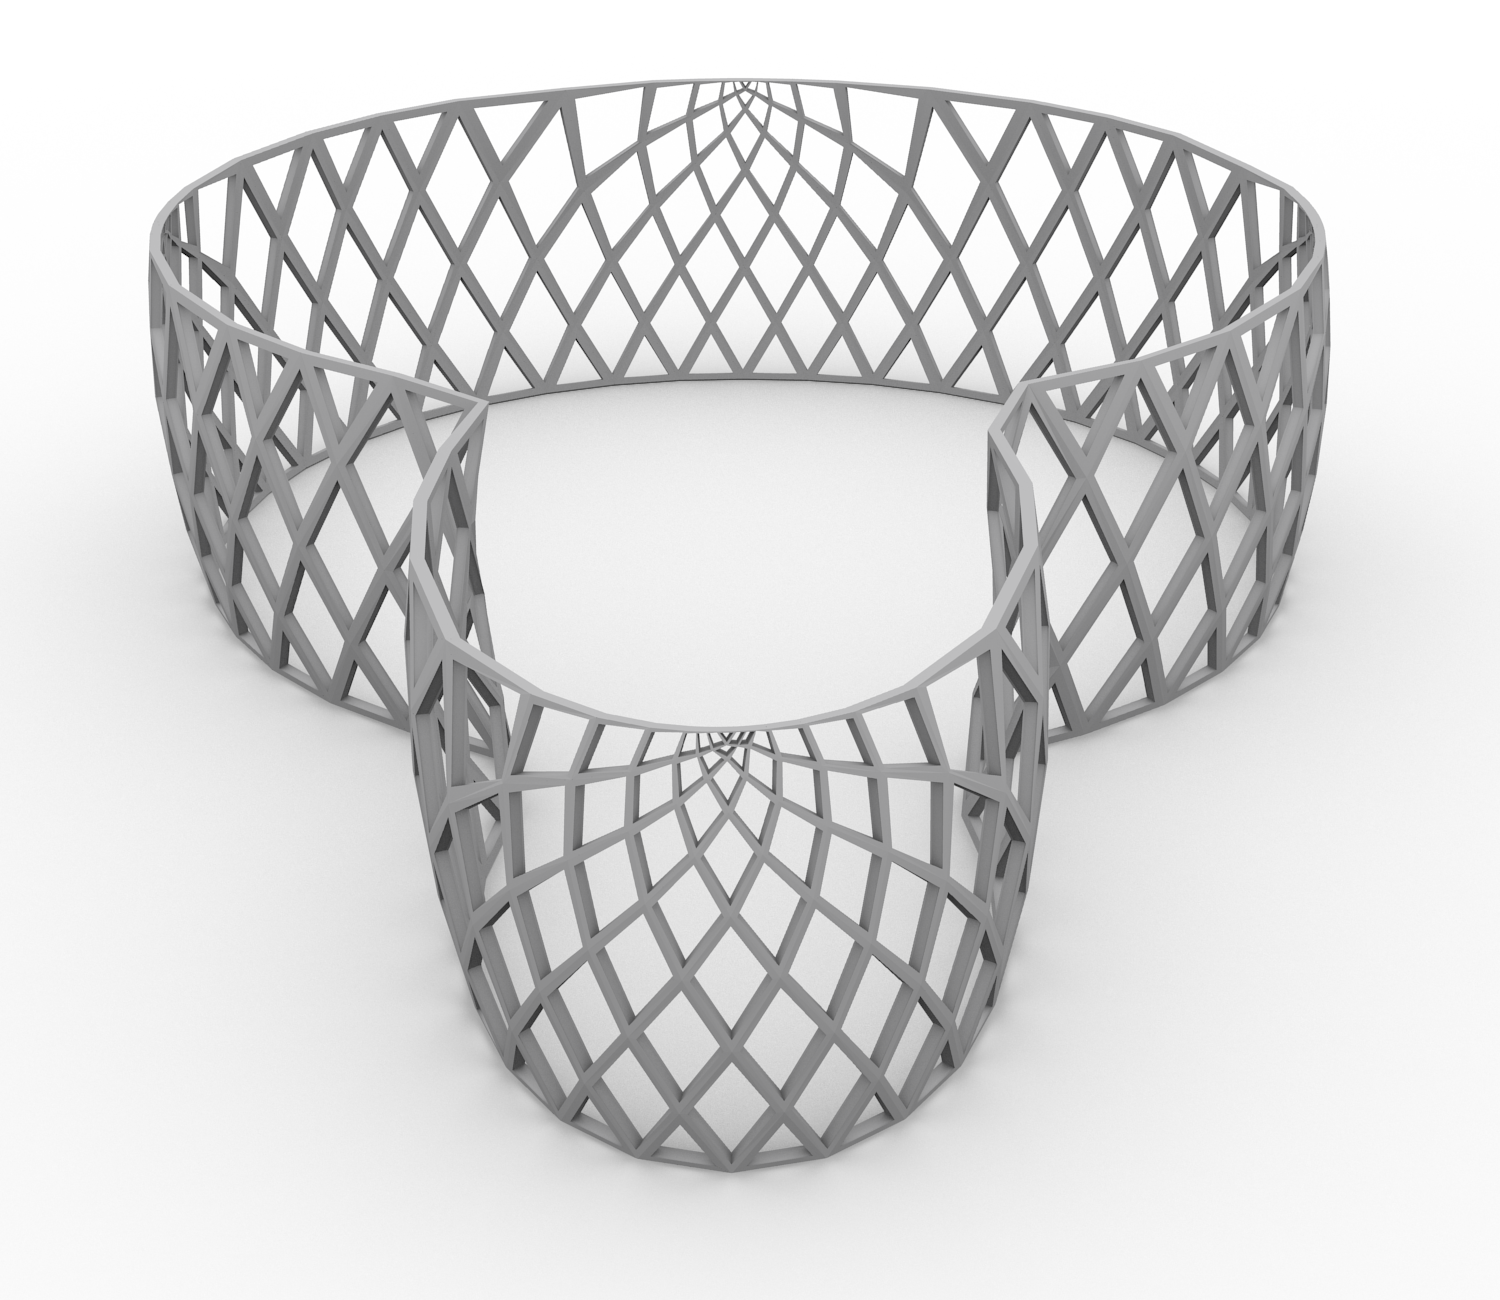
\includegraphics[width=.32\linewidth]{images/wanda_diagrid2.png}
  \caption{A periodic conformal map onto a cylinder with special
    vertices creates the opportunity to incorporate entrances (left)
    or concentration of support structure (right).}
  \label{fig:entrance}
\end{figure}

\subsubsection{Design and structural opportunities.}
Opposed to achieving a homogenous pattern distribution, as described
previously, it is also possible to use special boundary conditions to
support structural purposes or design requirements. If one aims for a
panelization with boundary aligned patterns, then the target boundary
angles must be quantized.

To include entrances in a facade it is possible to incorporate special 
boundary conditions. An example with special boundary vertices with domain angles
$\frac{4}{3}\pi$ and $\tfrac{\pi}{3}$ is shown in
Figure~\ref{fig:entrance}, left. In the remeshed surface, the lower boundary
curve bends inside at the vertices with angle~$\tfrac{4}{3}\pi$ around
the vertex with angle~$\tfrac{\pi}{3}$. This incorporates a natural
entrance into the facade.

Another effect of such angle conditions is a densification of the
pattern at the vertices with small angles. Such a concentration of
elements can be used to enforce structural properties of a
geometry. An example of a diagrid generated with such boundary
conditions is shown in Figure~\ref{fig:entrance}, right.

\end{document}

%%% Local Variables: 
%%% mode: latex
%%% TeX-master: "article"
%%% End: 
